\documentclass[12pt]{article}

% Packages
\usepackage[utf8]{inputenc}
\usepackage{amsmath,amsfonts,amssymb}
\usepackage{geometry}
\usepackage{graphicx}
\usepackage{enumitem}
\usepackage{placeins}
\usepackage{hyperref}
\usepackage{listings}
\usepackage{xcolor}
\usepackage{caption}
\usepackage{comment}
\usepackage[normalem]{ulem}
\geometry{a4paper, margin=1in}
\newcommand{\kt}{\texttt{kthread }}
\newcommand{\ut}{\texttt{uthread }}



\begin{document}

\title{
    \textmd{\textbf{CS4210\\TinyFile}}\\
    \vspace{0.1in}\small{March 2024}\\
}
\author{
    \begin{tabular}[t]{cc}
        \textbf{Eduardo Sanchez Rodriguez} & \textbf{Alberto Molina Felipe} \\
        \texttt{esanchez63@gatech.edu} & \texttt{afelipe3@gatech.edu} \\
    \end{tabular}
}

\date{}
\maketitle

% **************************************************** OVERALL DESIGN
\section*{Overall Design}

\subsection*{Understanding the Project}
\par The project is analogous to the implementation of domains in Xen. The tinyfile service works like \texttt{Dom0}, while each instance of the library in the apps are the different domains. We implemented a single queue for requests to the service and a response queue for each domain to receive responses from the service. Once the connection is established, a ring buffer in shared memory shephered to and from \texttt{Dom0}.

\subsection*{Message Queues}

\par At startup, the service creates the shared memory chunks given the arguments and the main message queue. Under the \texttt{'/tinyservice'} message queue library instances can push 3 type of messages:
\begin{itemize}
    \item \textit{Init}. When the app calls \texttt{init\_communication()} a message is sent with the process identifier, with the intention of keeping track of all instances for quality of service.
    \item \textit{Compress Request}. Every time an app wants to compress a file, this message serves as the request and it includes the pid to identify the request. 
    \item \textit{End}. When the app calls \texttt{end\_communication()}, tells the service that this instance won't be making anymore requests.
\end{itemize}


\par Once a library instance send a compress request in the main message queue it waits in its own queue \texttt{'/<pid>'}. When the service responds to a request it will send a message in this individual queue with the information requires to start the shared memory communication. The message contains how many message chunks and their size.

\newpage
\subsection*{Shared Memory}

\par At startup, the service allocates the shared memory chunks. Each chunk includes a mutex, condition variable, 2 integers and \texttt{sms\_size} bytes to communicate.

\par The mutex and condition variable serve a clear purpose, allow for exclusive access to the writable bytes in the chunk. The integers are specific to the tinyfile service.

\par The first integer in the chunk refers to the status and the other to the bytes written. We differentiated the possible contents of the chunk in raw/uncompressed data, compressed data and empty. Given those states the status of each chunk can be: \textit{empty}, \textit{raw}, \textit{compressed}, \textit{done\_lib} when its uncompressed and the library finished copying into shared memory and \textit{done\_ser} when its compressedand the service finished compressing the last chunk.

\par Communication with shared memory looks like a state machine. In the following table we describe the response of the library instance in each state. Its options are: read \texttt{R} or write \texttt{W} into the chunk, move to the next one \texttt{++} or hold on the mutex \texttt{H}.

\begin{table}[h]
\centering
\begin{tabular}{|l|c|c|c|c|c|}
\hline
\multicolumn{1}{|c|}{} & \multicolumn{5}{c|}{Chunk Status} \\ \hline
Library State & Empty & Raw & Compressed & Done Lib & Done Ser\\ \hline
Copying raw file & \texttt{W ++} & \texttt{H} & \texttt{R W ++}   & \texttt{-} & \texttt{-} \\
Finished copying & \texttt{++}   & \texttt{H} & \texttt{R ++}     & \texttt{H} & \texttt{R finish} \\ \hline
\end{tabular}
\end{table}


\par When it writes uncompressed bytes into the chunk it changes its status to \textit{raw}, if it happens to be its last chunk of bytes to write the status is changed to \textit{done\_lib} and it also signals how many bytes it has written, in case it doesn't fill the whole chunk.

\par The policy for the service is a lot simpler. It can hold, move one and compressed the chunks \texttt{Z}.When it compresses a chunk it always writes how many bytes it has written. If it compresses the chunk with status \textit{done\_lib} it 


\begin{table}[h]
\centering
\begin{tabular}{|c|c|c|c|c|}
\hline
\multicolumn{5}{|c|}{Chunk Status} \\ \hline
Empty & Raw & Compressed & Done Lib & Done Ser\\ \hline
\texttt{H} & \texttt{Z} & \texttt{H} & \texttt{Z finish} & \texttt{-} \\ \hline
\end{tabular}
\end{table}

\par We can illustrate some possible scenarios with the following diagrams. At first, the state of the shared memory array of chunks may look something like this. The library has written some raw chunks and the serviceis compressing the first chunk the library has written.

\begin{figure}[h]
\centering
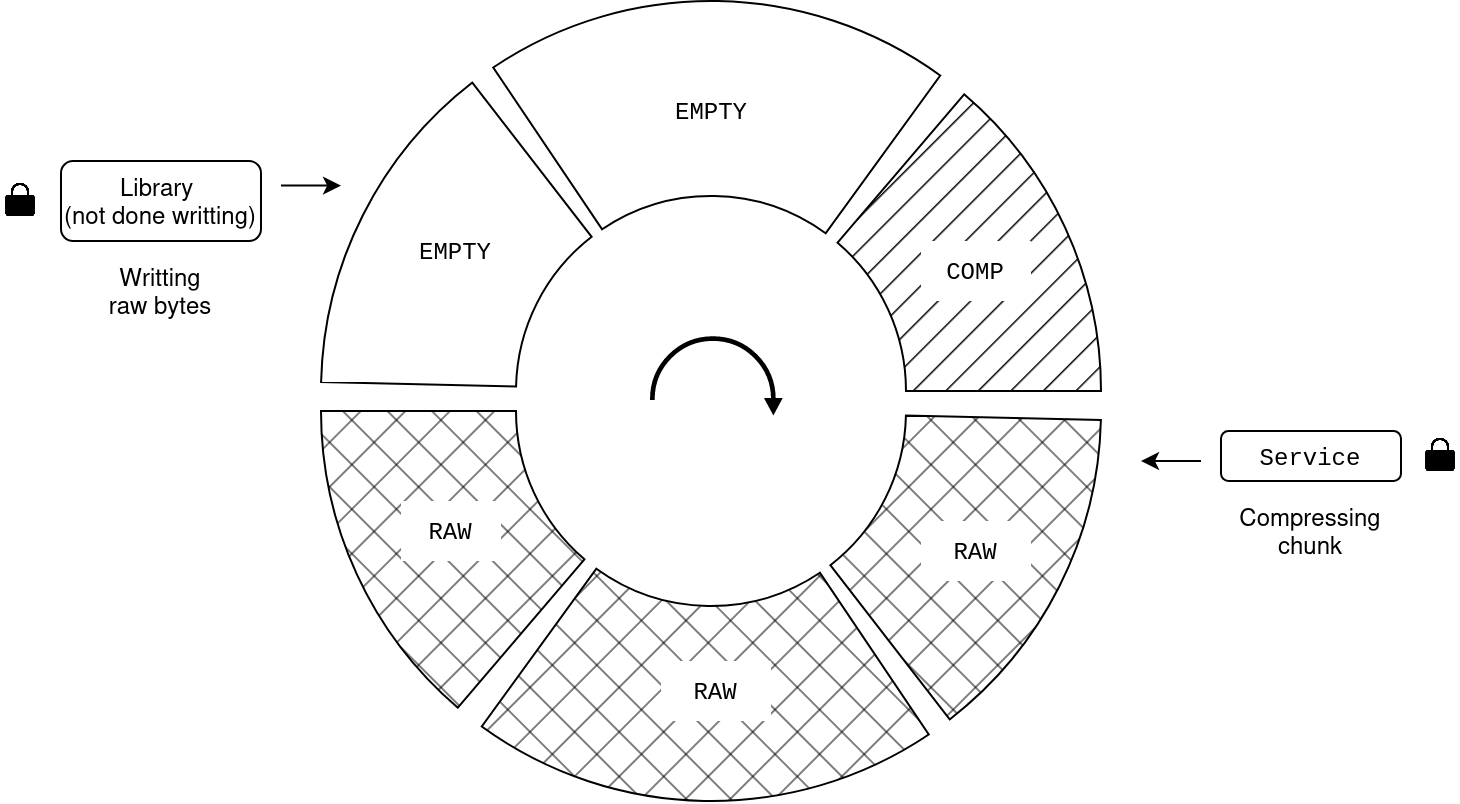
\includegraphics[width=0.6\textwidth]{AOS-start.png}
\end{figure}
\FloatBarrier

\newpage
\par In one scenario, the library had written its last raw chunk into the shared memory, and it moves to the first compressed chunk and copies its content to the output file. In this case, the service has taken longer to work around the circular buffer and has the mutex of the last chunk of raw bytes while the library has copied all the compressed bytes and is waiting to get the mutex.

\begin{figure}[h]
\centering
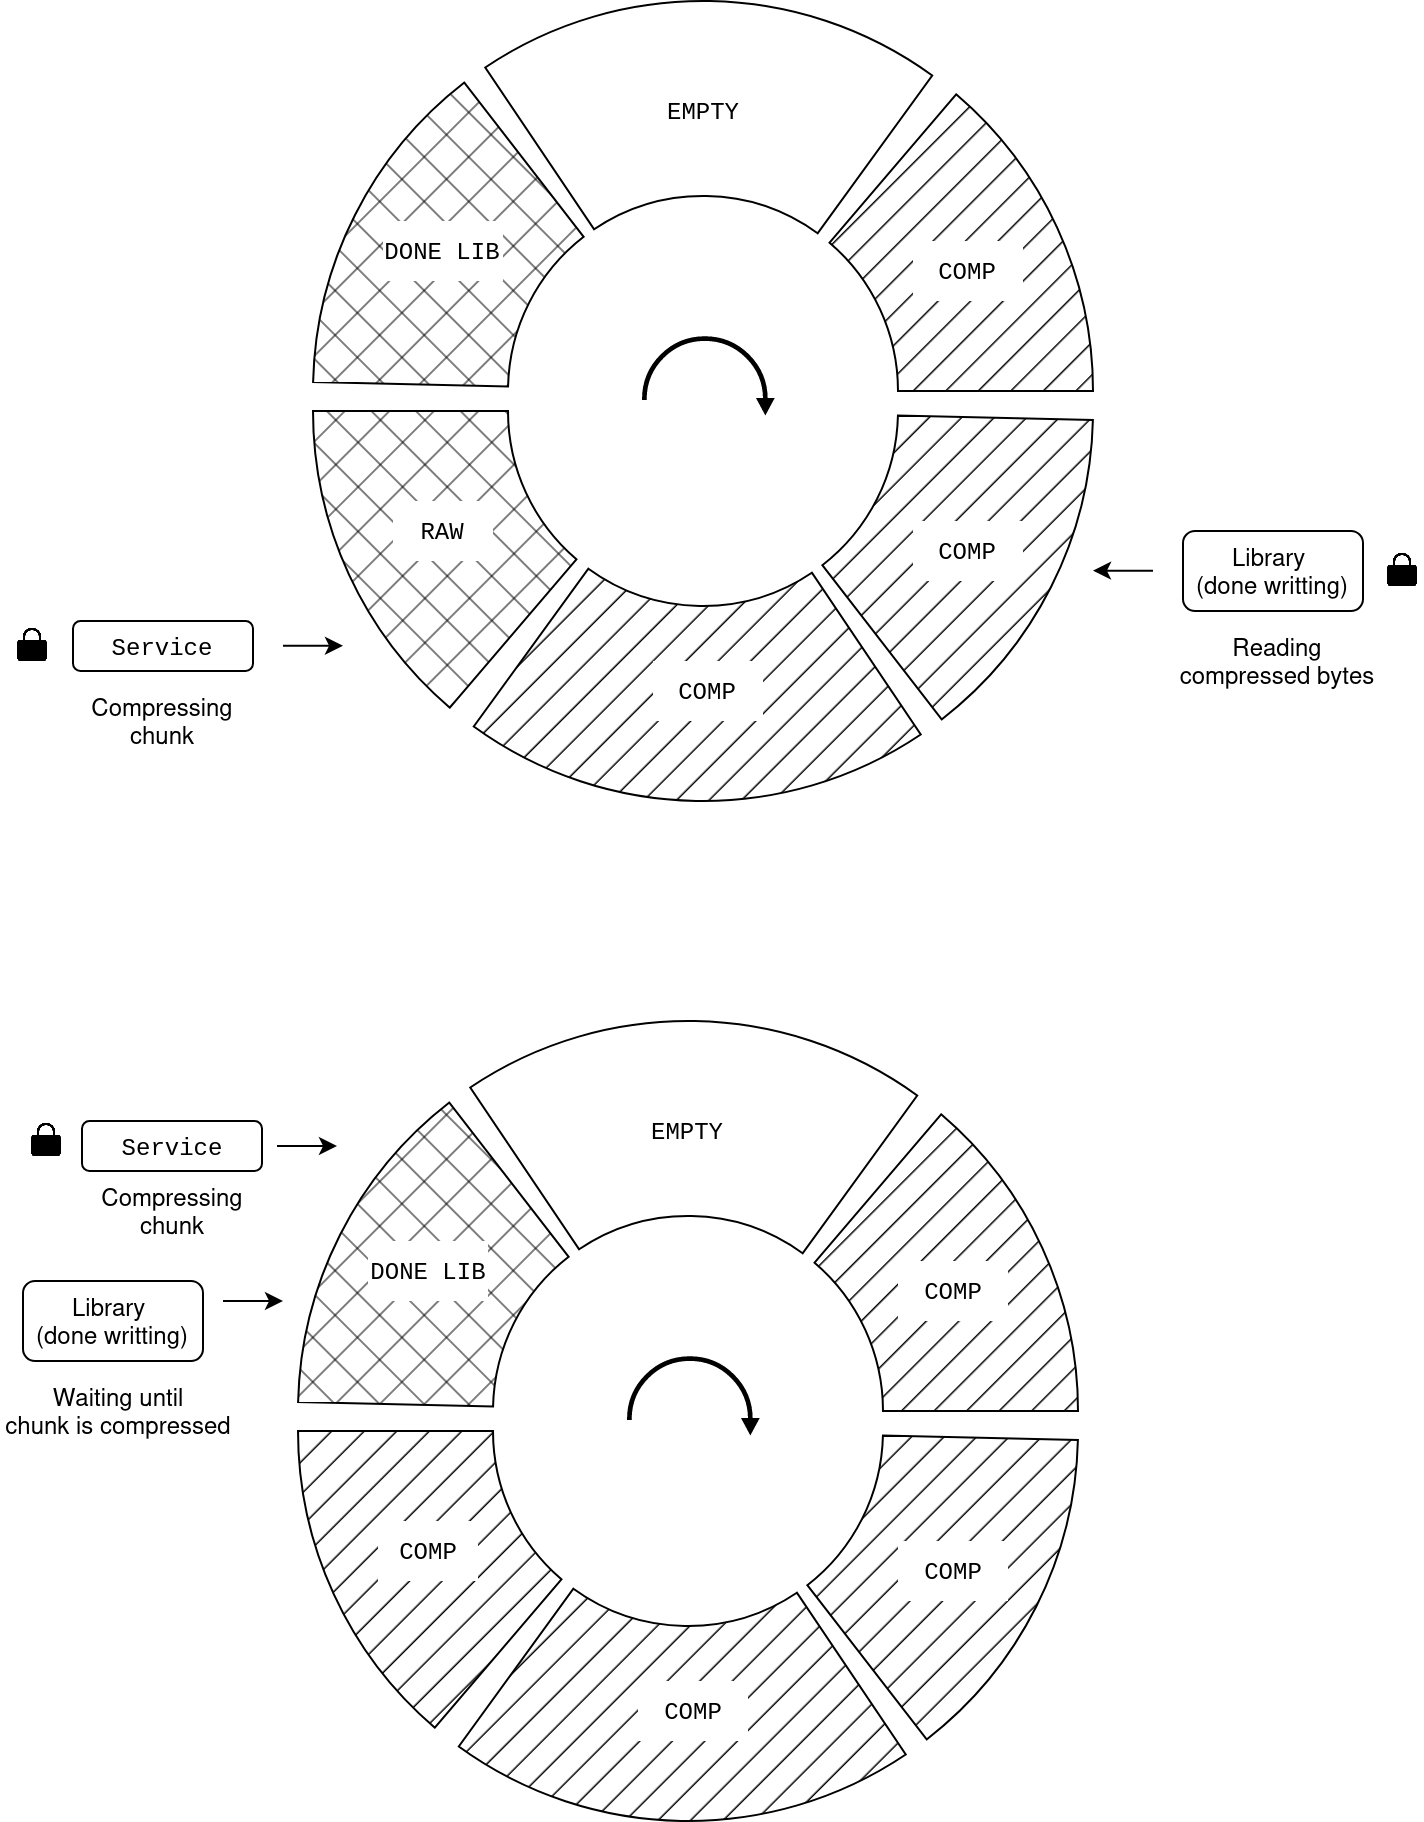
\includegraphics[width=0.9\textwidth]{AOS-done.png}
\end{figure}
\FloatBarrier


\newpage
\par In a second scenario, the library is compressing a larger file and it's not done copying the raw bytes.
The library has gone around each compressed chunk, reading its contents into the output file and writing the raw bytes.
Here, for scheduling or faster compression, the service has caught up to the library and is waiting on the mutex while the library is processing the compressed chunk.
\begin{figure}[h]
\centering
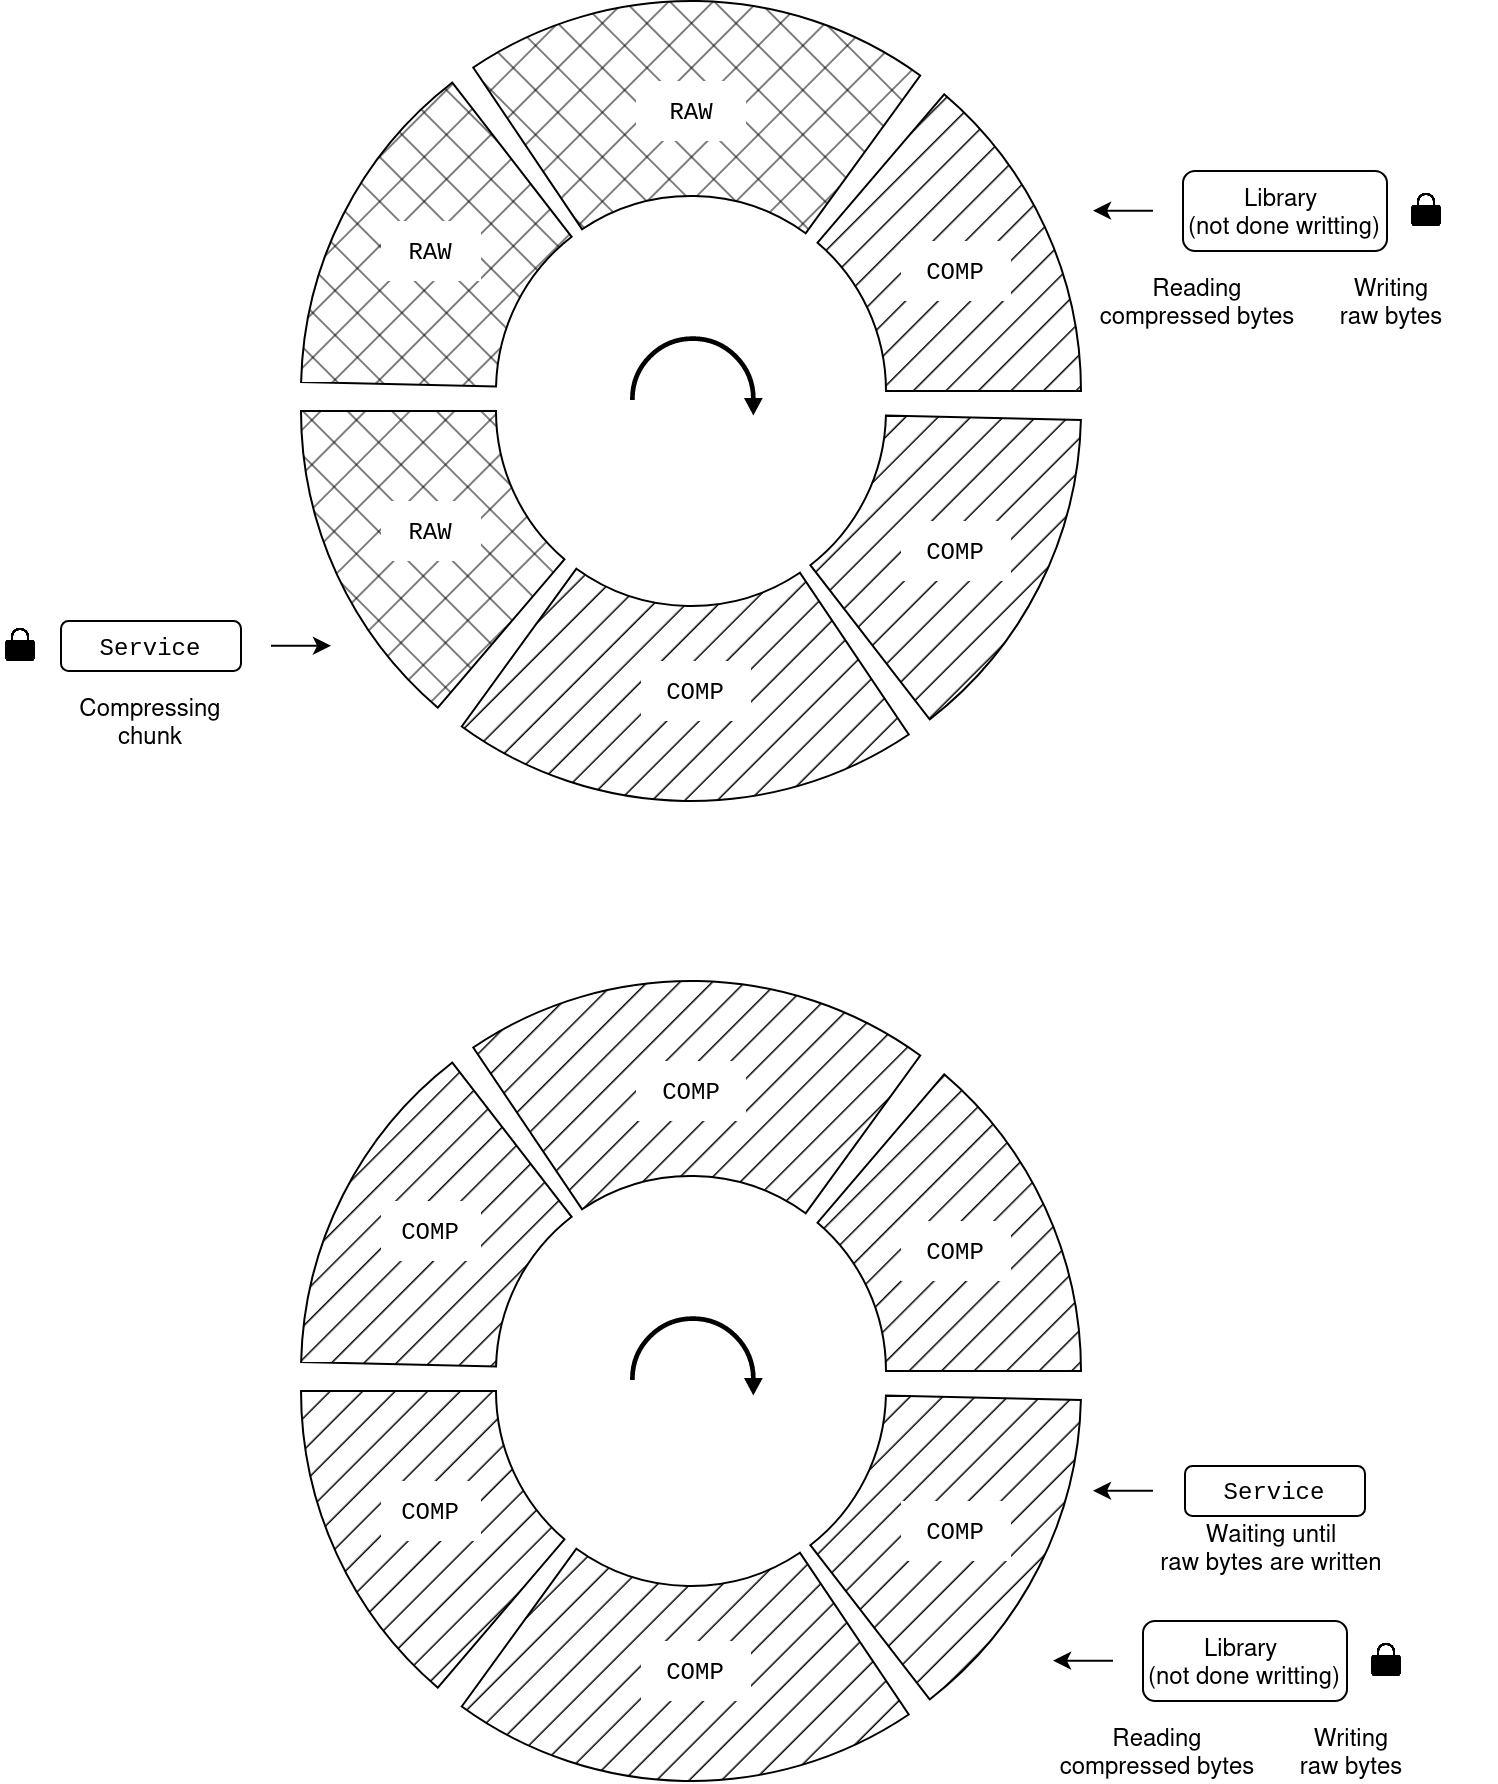
\includegraphics[width=0.9\textwidth]{AOS-not-done.png}
\end{figure}
\FloatBarrier


% **************************************************** SYNC / ASYNC
\section*{Sync/Async Implementation}



% **************************************************** EXPERIMENT 
\section*{Experiment}



% **************************************************** QOS 
\section*{Quality of Service}
\par We implemented QoS in our project by prioritizing tasks based on the number of requests fulfilled, despite the alternative of designing our approach around the volume of bytes processed.

\par Prioritizing clients based on request count rather than data size might not reflect the true resource consumption or prioritize critical larger requests, potentially leading to overlooked client needs. However, this approach aims to ensure equitable service access and prevent a few clients with small and frequent requests from dominating resources.

\par When an app wants to use the service it must initialize communication, letting the server know there is one more thread that wants to compress files. The service keeps a linked list to keep count of how many request each process has made and if its waiting for a response. 

% **************************************************** LOGS
\section*{Logs}



% **************************************************** PRINTS
\section*{Figures}



\end{document}
